\documentclass[simplex.tex]{subfiles}
% NO NEED TO INPUT PREAMBLES HERE
% packages are inherited from simplex.tex; you can compile this on its own
\begin{document}
\subsection{ndreg}
%% Jan

We received three new CLARITY image volumes from our colleagues at Stanford University. 
Each dataset contained two channels of a single mouse brain hemisphere at a 585 $\mu m$ $\times$ 585 $\mu m$ $\times$ 5000 $\mu m$ resolution.
The images were ingested and propagated to lower resolutions using NeuroData infrastructure.
NeuroData's registration module (ndreg) was then used to register each image to the Allen institute's mouse Reference Atlas (ARA).

First each image was reoriented to the ARA, the background was subtracted and a mask was generated to eliminate bright regions.
After affine alignment, each Stanford image was deformably aligned to the ARA through Large Deformation Diffeomorphic Metric Mapping (LDDMM).
Since the ARA and CLARITY images differed greatly in intensity profile, mutual information matching was adopted during this step.
Alignment was done in a 3-step multi-resolution approach, with registration at coarser scales initializing the alignment at subsequent finer scales.
It was clear from the ARA-CLARITY checkerboard composite images that registration proceeded successfully (Figure~\ref{fig:ndregAiley}).

\begin{figure}[h!]
\begin{cframed}
\centering
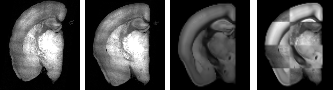
\includegraphics[width=0.75\textwidth]{../../figs/ndreg-ailey.png}
\caption{
  Coronal slices from image volumes.
  From left to right: CLARITY before LDDMM, CLARITY after LDDMM, ARA, checkerboard composite of ARA and CLARITY after LDDMM.
}
\label{fig:ndregAiley}
\end{cframed}
\end{figure}

\clearpage

%% Feb
The NeuroData Registration python module, \textit{ndreg}, uses \textit{Large Deformation Diffeomorphic Metric Mapping (LDDMM)} to register a template image $I_0$ to a target image $J_1$.
It does this by finding smooth invertible map $\varphi$ such that the \textit{matching term} $M(I_0 \circ \varphi^{-1}, J_1)$, a function whose value is small when $I_0 \circ \varphi^{-1}$ is aligned with $J_1$, is minimized.
We compared MI-LDDMM, LDDMM with a Mutual Information based matching term, to our previous SSD-LDDMM and Mask-LDDMM techniques.
SSD-LDDMM uses a Sum of Squared Differences matching term.
As it is based on image subtraction, it assumes that bright regions in $I_0$ align with bright regions in $J_1$.
Mask-LDDMM is SSD-LDDMM in which $I_0$ and $J_1$ are replaced with their respective binary brain mask images $M_0$ and $M_1$.
Since the masks only contain information on which voxels are inside the brain, only edge information is used by Mask-LDDMM.
\\
We placed fiducial landmarks in the corpus callosum and midbrain of four CLARITY template image and the \textit{Allen Reference Atlas (ARA)} target.
After registration corresponding CLARITY landmarks should be close to those of the ARA. 
If not then the registration was inadequate.
Figure~\ref{fig:comparison} shows that MI-LDDMM registration performed better than the previous methods.

\begin{figure}[!h]
\begin{cframed}
\centering
 \begin{subfigure}{0.25\columnwidth}
  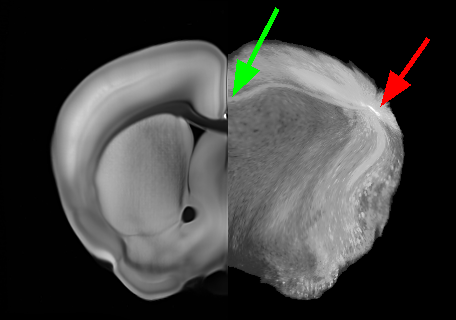
\includegraphics[width=\textwidth]{../../figs/ssdCoronal.png}  
  \caption{SSD-LDDMM}
  \label{fig:clarityCoronalSSD}
 \end{subfigure}
 \begin{subfigure}{0.25\columnwidth}
  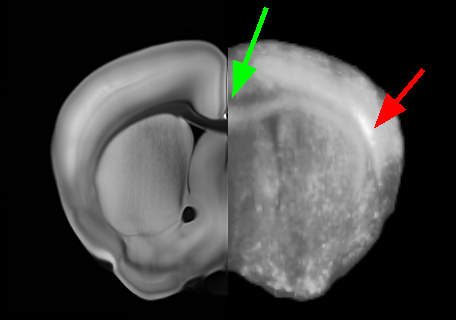
\includegraphics[width=\textwidth]{../../figs/maskCoronal.png}  
  \caption{Mask-LDDMM}
  \label{fig:clarityCoronalMask}
 \end{subfigure}
 \begin{subfigure}{0.25\columnwidth}
  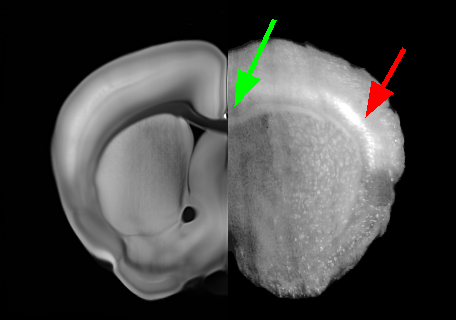
\includegraphics[width=\textwidth]{../../figs/miCoronal.png}  
  \caption{MI-LDDMM}
  \label{fig:clarityCoronalMI}
 \end{subfigure}
 \begin{subfigure}{0.2\columnwidth}
  %\captionsetup{justification=centering} % Center caption
  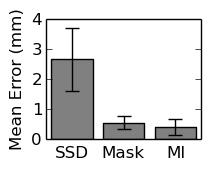
\includegraphics[width=\textwidth]{../../figs/lmkError.png}  
  \caption{Landmark Error}
  \label{fig:lmkError}
 \end{subfigure}
 \caption{Comparison of SSD-LDDMM (\subref{fig:clarityCoronalSSD}), Mask-LDDMM (\subref{fig:clarityCoronalMask}) and MI-LDDMM (\subref{fig:clarityCoronalMI}) registration for a CLARITY mouse brain.
  Panes (\subref{fig:clarityCoronalSSD}-\subref{fig:clarityCoronalMI}) have an ARA coronal slice on the left juxtaposed to the corresponding aligned CLARITY slice on the right.
  Green arrows point out that the corpus callosum is misaligned by SSD-LDDMM but aligned correctly by MI matching.
  Red arrows show that SSD-LDDMM distorts bright regions.
  Fiducial landmarks were placed throughout the corpus callosum, and midbrain of the acquired volumes.
  Pane (\subref{fig:lmkError}) compares mean errors between the deformed CLARITY and ARA landmarks after registration.
 }
 \label{fig:comparison}
\end{cframed}
\end{figure}

\clearpage

%% March
We received a rat brain image acquired using iDISCO microscopy from colleagues at the Johns Hopkins School of Medicine. 
iDISCO is a technique for clearing tissues that enables interrogatoion by light-sheet microscopy. 
Thus like CLARITY, iDISCO cleared brains can be imaged at high spatial resolution without physical slicing.
The iDISCO volume was ingested into the NeuroData store at its full resolution of 5 $\mu$m isotropic.
We also ingested the widely used Waxholm Rat Atlas, a T2 magnetic resonance image with corresponding labels at a 39 $\mu$m isotropic.\\

\textit{Large Deformation Diffeomorphic Metric Mapping (LDDMM)} is a deformable image registration (alignment) algorithm which computes smooth invertible transforms between images.
Using the \textit{NeuroData Registration (ndreg)} python module we were able to perform a iDISCO to T2 MRI alignment by LDDMM under mutual information matching.
Figure~\ref{fig:idisco} shows the Waxholm Rat Atlas labels overlaid on the iDISCO image.

\begin{figure}[!h]
 \begin{cframed}
  \centering
   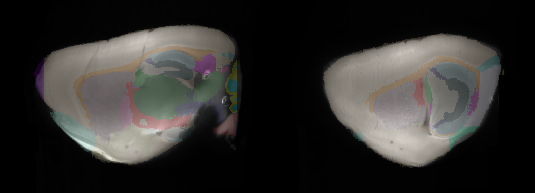
\includegraphics[width=\textwidth]{../../figs/iDISCO.png}  
   \caption{Waxholm rat atlas labels overlaid on sagittal slices of iDISCO rat brain}
  \label{fig:idisco}
 \end{cframed}
\end{figure}

\clearpage
\end{document}
